% !TEX root = MusicFormatsUserGuide.tex

% -------------------------------------------------------------------------
\chapter{MusicFormats installation modes}
% -------------------------------------------------------------------------

There is no GUI installer available yet, so users have to install the library at a lower level, sorry for that\dots.

How to install \mf\ depends on the \OS. \Linux\ users often build the software they use themselves, while those of \Windows\ and \MacOS\ are accustomed to install in much simpler ways.

Depending on the needs, users may wish to install the \MainIt{whole} \mf\ with source code and examples, or to use a \MainIt{distribution}, that contains only the \MainIt{libraries} if relevant, the \CLI\ executables and the documentation \pdf\ files.

The following chapters show the details.


% -------------------------------------------------------------------------
\chapter{Using a distribution}
% -------------------------------------------------------------------------

\mf\ comes with distributions for \MacOS, \Ubuntu\ and \Windows\ in the form of \zip\ files., including the user documentation PDF file. \fileName{MusicFormatsVersionNumber.txt} contains the library's version number:
\begin{lstlisting}[language=Terminal]
jacquesmenu@macmini: ~/musicformats_local_clone/distrib > ls -sal
total 150088
     0 drwxr-xr-x   8 jacquesmenu  staff       256 Feb 16 07:47 .
     0 drwxr-xr-x  22 jacquesmenu  staff       704 Feb 16 07:47 ..
  1672 -rw-r--r--   1 jacquesmenu  staff    854294 Feb 16 07:47 IntroductionToMusicXML.pdf
  1976 -rw-r--r--   1 jacquesmenu  staff   1008702 Feb 16 07:47 MusicFormatsUserGuide.pdf
108168 -rw-r--r--   1 jacquesmenu  staff  55378423 Feb 16 07:47 MusicFormatsForMacOS.zip
 34080 -rw-r--r--   1 jacquesmenu  staff  17445663 Feb 16 07:47 MusicFormatsForUbuntu.zip
  4184 -rw-r--r--   1 jacquesmenu  staff   2139537 Feb 16 07:47 MusicFormatsForWindows.zip
     8 -rw-r--r--   1 jacquesmenu  staff         6 Feb 16 07:47 MusicFormatsVersionNumber.txt
\end{lstlisting}

The distributions \zip\ archives are supplied with all versions, i.e. the current, most recent version of \mf (the default branch in the \repo), and the earlier versions such as the \code{v0.9.60} branch.


% -------------------------------------------------------------------------
\section{MacOS\texttrademark\ distribution}
% -------------------------------------------------------------------------

\MacOS\ software is usually distributed as \Main{DMG} files. Due to file size limitations on \github, the \MacOS\ distribution has to be compacted. This is done with \zip, and placing that in a DMG archive would not add any value. Only the \zip\ archive is thus provided.

%%%JMI\mf\ is  installable directly from the repository, since this is the environment is is developed on. Just clone the \repo\ and you will find the executables in \build{bin} and the libraries in \build{lib}.

After downloading and uncompressing \fileName{MusicFormatsForMacOS.zip}, we get:
\begin{lstlisting}[language=Terminal]
jacquesmenu@macmini: ~/Downloads/MusicFormatsForMacOS > ls -sal *
8 -rw-r--r--@ 1 jacquesmenu  staff  6 Feb 14 14:20 MusicFormatsVersionNumber.txt

bin:
total 661992
    0 drwxr-xr-x@ 25 jacquesmenu  staff       800 Feb 14 14:20 .
    0 drwxr-xr-x@  4 jacquesmenu  staff       128 Feb 15 17:23 ..
74864 -rwxr-xr-x@  1 jacquesmenu  staff  38326752 Feb 14 14:20 LilyPondIssue34
74864 -rwxr-xr-x@  1 jacquesmenu  staff  38329824 Feb 14 14:20 Mikrokosmos3Wandering
 8432 -rwxr-xr-x@  1 jacquesmenu  staff   4314896 Feb 14 14:20 MusicAndHarmonies
 8432 -rwxr-xr-x@  1 jacquesmenu  staff   4314880 Feb 14 14:20 RandomChords
 8432 -rwxr-xr-x@  1 jacquesmenu  staff   4314880 Feb 14 14:20 RandomMusic
 8624 -rwxr-xr-x@  1 jacquesmenu  staff   4414944 Feb 14 14:20 countnotes
16528 -rwxr-xr-x@  1 jacquesmenu  staff   8459424 Feb 14 14:20 displayMusicformatsHistory
16528 -rwxr-xr-x@  1 jacquesmenu  staff   8459424 Feb 14 14:20 displayMusicformatsVersion
79200 -rwxr-xr-x@  1 jacquesmenu  staff  40546384 Feb 14 14:20 msdlconverter
12480 -rwxr-xr-x@  1 jacquesmenu  staff   6387232 Feb 14 14:20 partsummary
 8848 -rwxr-xr-x@  1 jacquesmenu  staff   4528736 Feb 14 14:20 readunrolled
64000 -rwxr-xr-x@  1 jacquesmenu  staff  32764496 Feb 14 14:20 xml2brl
66872 -rwxr-xr-x@  1 jacquesmenu  staff  34236240 Feb 14 14:20 xml2gmn
17160 -rwxr-xr-x@  1 jacquesmenu  staff   8781984 Feb 14 14:20 xml2guido
67552 -rwxr-xr-x@  1 jacquesmenu  staff  34583840 Feb 14 14:20 xml2ly
12392 -rwxr-xr-x@  1 jacquesmenu  staff   6342528 Feb 14 14:20 xml2midi
59720 -rwxr-xr-x@  1 jacquesmenu  staff  30574528 Feb 14 14:20 xml2xml
 9104 -rwxr-xr-x@  1 jacquesmenu  staff   4657200 Feb 14 14:20 xmlclone
 9256 -rwxr-xr-x@  1 jacquesmenu  staff   4735296 Feb 14 14:20 xmlfactory
 8800 -rwxr-xr-x@  1 jacquesmenu  staff   4504976 Feb 14 14:20 xmliter
 8680 -rwxr-xr-x@  1 jacquesmenu  staff   4442496 Feb 14 14:20 xmlread
11976 -rwxr-xr-x@  1 jacquesmenu  staff   6129744 Feb 14 14:20 xmltranspose
 9248 -rwxr-xr-x@  1 jacquesmenu  staff   4734368 Feb 14 14:20 xmlversion
\end{lstlisting}

\MacOS\ executables are self-sufficient and can be placed anywhere on a disk except the trash. Usually, there are placed in the \code{/Applications} directory.


% -------------------------------------------------------------------------
\subsection{Security issue in recent MacOS\texttrademark\ versions}
% -------------------------------------------------------------------------

\MacOS\ gets more and more stringent over time regarding security. The \OS\ part in charge of this is named \Gatekeeper.

When installing \mf\ from the \repo\ on versions up to 10 (\Main{High Sierra}), the executables in \code{bin} are usable alright.

From version 11 (\Main{Catalina}) on, though, the executables you get are not executable actually, because their developer is unknown to the \OS, and actions have to be taken for them to be usable.

The screenshot below has been made with \MacOS\ \Main{Monterey} 12.0.1 with english as the user interface language. The texts vary of course depending on the language used.

When launching one of these executables for the first time, such as:
\begin{lstlisting}[language=Terminal]
jacquesmenu@macmini: ~/Downloads/MusicFormatsForMacOS/bin > ./xml2ly
\end{lstlisting}
we get a alert telling that it cannot be opened, because the developper is not known to the \OS:\\
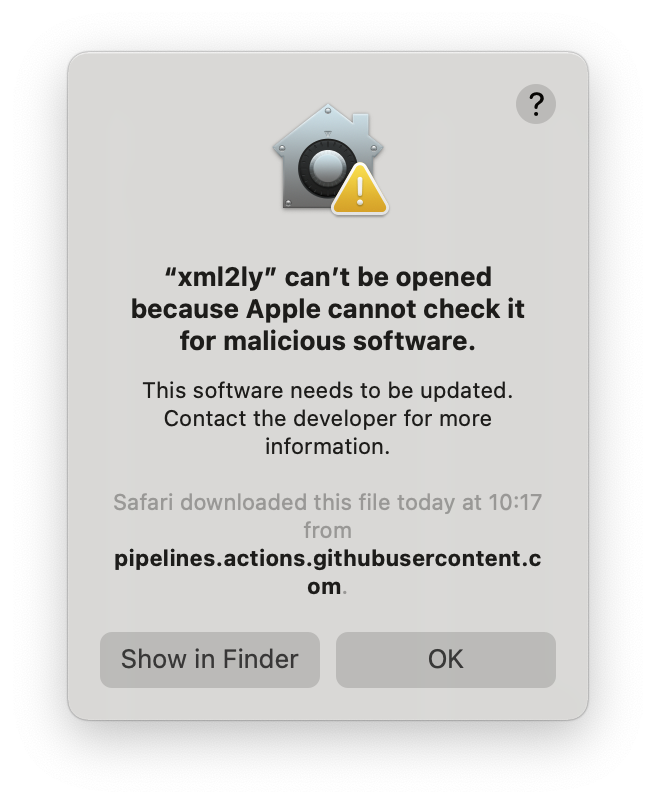
\includegraphics[scale=0.35]{../graphics/MacOSMaliciousSoftwareAlert.png}

Clicking in either buttons in this dialog kill the process:
\begin{lstlisting}[language=Terminal]
Killed: 9
\end{lstlisting}

The trouble is that these executables are in {\it \quarantine} by default. To make them usable, they have to quit quarantine, which is done by removing one of their attributes:
\begin{lstlisting}[language=Terminal]
jacquesmenu@macmini: ~/Downloads/MusicFormatsForMacOS/bin > xattr -d com.apple.quarantine *
\end{lstlisting}
%codesign --sign - --force --deep %%%JMI not necessary

From then on, the \mf\ executables can be used seamlessly on the given machine.

Having to perform the preceding task for each executable is the price to pay for security. And it has to be perfomed again when installing new versions\dots


The above can be done in the \GUI\ file by file too. Right after you got the message above:
\begin{itemize}
\item  open \MainIt{System Preferences}, choose the \MainIt{Security \& Privacy} tab, and there click on the \MainIt{General button};

\item click on the lock at the bottom left of the dialog to make changes:\\
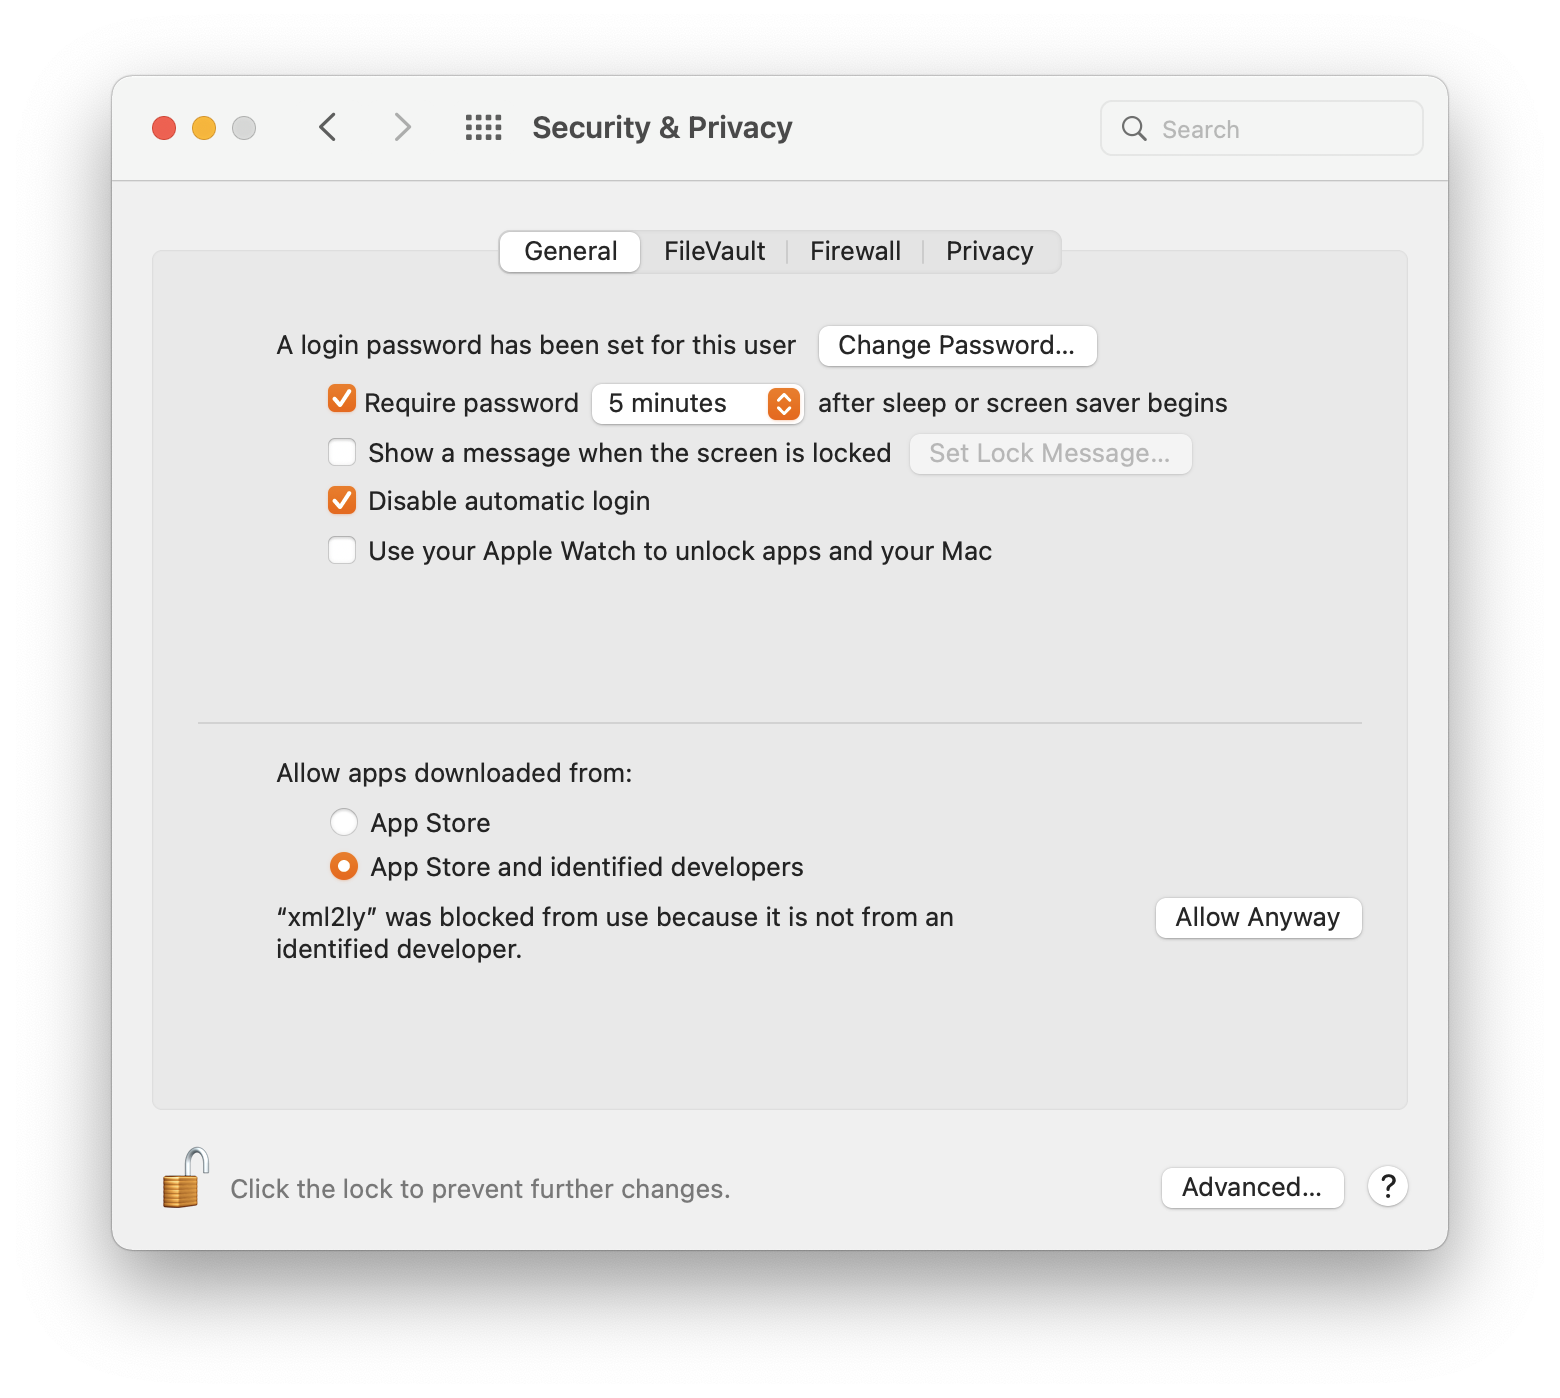
\includegraphics[scale=0.35]{../graphics/MacOSAllowAnyway.png}

\item click on the \MainIt{Allow Anyway} button.
%%%JMI sudo spctl --master-disable to create a Anywhere radio button
%jacquesmenu@macmini > spctl --status
%assessments enabled

\end{itemize}

Re-execute the executable from the command line. This pops-up a dialog to confirm you actually want to use this software:\\
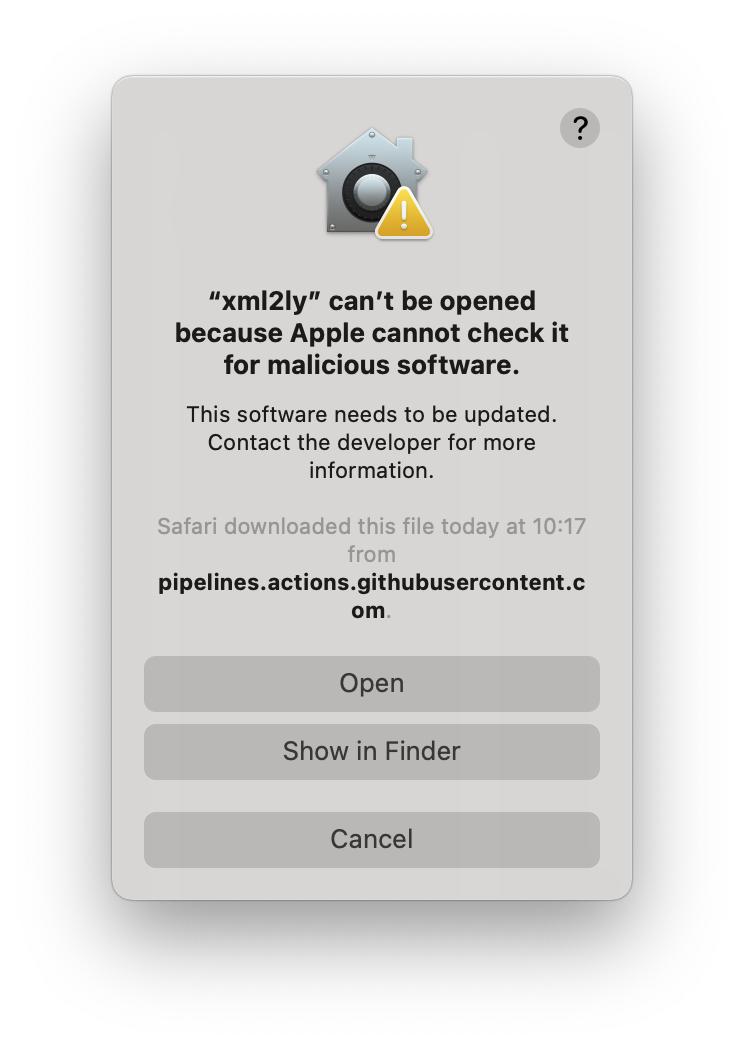
\includegraphics[scale=0.35]{../graphics/MacOSConfirmOpening.png}

Click on the \MainIt{Open} button to register the executable in \Gatekeeper\ and go ahead.


% -------------------------------------------------------------------------
\section{Ubuntu distribution}
% -------------------------------------------------------------------------

After downloading, we get:
\begin{lstlisting}[language=Terminal]
jacquesmenu@macmini: ~/Downloads/MusicFormatsForUbuntu > ls -sal *
8 -rw-r--r--@ 1 jacquesmenu  staff  6 Feb 14 14:33 MusicFormatsVersionNumber.txt

bin:
total 2296
  0 drwxr-xr-x@ 25 jacquesmenu  staff     800 Feb 14 18:22 .
  0 drwxr-xr-x@  6 jacquesmenu  staff     192 Feb 16 08:45 ..
 96 -rw-r--r--@  1 jacquesmenu  staff   49000 Feb 14 14:33 LilyPondIssue34
 96 -rw-r--r--@  1 jacquesmenu  staff   49040 Feb 14 14:33 Mikrokosmos3Wandering
 96 -rw-r--r--@  1 jacquesmenu  staff   47224 Feb 14 14:33 MusicAndHarmonies
 96 -rw-r--r--@  1 jacquesmenu  staff   47216 Feb 14 14:33 RandomChords
 96 -rw-r--r--@  1 jacquesmenu  staff   47216 Feb 14 14:33 RandomMusic
 72 -rw-r--r--@  1 jacquesmenu  staff   33800 Feb 14 14:33 countnotes
 40 -rw-r--r--@  1 jacquesmenu  staff   17648 Feb 14 14:33 displayMusicformatsHistory
 40 -rw-r--r--@  1 jacquesmenu  staff   17648 Feb 14 14:33 displayMusicformatsVersion
104 -rw-r--r--@  1 jacquesmenu  staff   50616 Feb 14 14:33 msdlconverter
544 -rw-r--r--@  1 jacquesmenu  staff  275976 Feb 14 14:33 partsummary
 88 -rw-r--r--@  1 jacquesmenu  staff   43720 Feb 14 14:33 readunrolled
 80 -rw-r--r--@  1 jacquesmenu  staff   39200 Feb 14 14:33 xml2brl
 88 -rw-r--r--@  1 jacquesmenu  staff   43336 Feb 14 14:33 xml2gmn
 48 -rw-r--r--@  1 jacquesmenu  staff   23112 Feb 14 14:33 xml2guido
 80 -rw-r--r--@  1 jacquesmenu  staff   39056 Feb 14 14:33 xml2ly
 88 -rw-r--r--@  1 jacquesmenu  staff   42880 Feb 14 14:33 xml2midi
 88 -rw-r--r--@  1 jacquesmenu  staff   43344 Feb 14 14:33 xml2xml
 88 -rw-r--r--@  1 jacquesmenu  staff   43368 Feb 14 14:33 xmlclone
 48 -rw-r--r--@  1 jacquesmenu  staff   22616 Feb 14 14:33 xmlfactory
168 -rw-r--r--@  1 jacquesmenu  staff   83488 Feb 14 14:33 xmliter
 56 -rw-r--r--@  1 jacquesmenu  staff   28424 Feb 14 14:33 xmlread
 56 -rw-r--r--@  1 jacquesmenu  staff   28656 Feb 14 14:33 xmltranspose
 40 -rw-r--r--@  1 jacquesmenu  staff   17360 Feb 14 14:33 xmlversion

lib:
total 157792
     0 drwxr-xr-x@ 4 jacquesmenu  staff       128 Feb 14 18:22 .
     0 drwxr-xr-x@ 6 jacquesmenu  staff       192 Feb 16 08:45 ..
113224 -rw-r--r--@ 1 jacquesmenu  staff  57968176 Feb 14 14:33 libmusicxml2.a
 44568 -rw-r--r--@ 1 jacquesmenu  staff  22818696 Feb 14 14:33 libmusicxml2.so
\end{lstlisting}

Move the \fileName{MusicFormatsForUbuntu} directory to a suitable place and set your \code{PATH} and \code{LIBRARY_PATH} \environmentVariable s accordingly.


% -------------------------------------------------------------------------
\section{Windows\texttrademark\ distribution}
% -------------------------------------------------------------------------

After downloading, we get:
\begin{lstlisting}[language=Terminal]
jacquesmenu@macmini: ~/Downloads/MusicFormatsForWindows > ls -sal *
8 -rw-r--r--@ 1 jacquesmenu  staff  6 Feb 14 14:53 MusicFormatsVersionNumber.txt

bin:
total 1232
  0 drwxr-xr-x@ 25 jacquesmenu  staff    800 Feb 14 18:22 .
  0 drwxr-xr-x@  6 jacquesmenu  staff    192 Feb 16 08:49 ..
 80 -rw-r--r--@  1 jacquesmenu  staff  38400 Feb 14 14:53 LilyPondIssue34.exe
 80 -rw-r--r--@  1 jacquesmenu  staff  38400 Feb 14 14:53 Mikrokosmos3Wandering.exe
 56 -rw-r--r--@  1 jacquesmenu  staff  26112 Feb 14 14:53 MusicAndHarmonies.exe
 56 -rw-r--r--@  1 jacquesmenu  staff  25088 Feb 14 14:53 RandomChords.exe
 56 -rw-r--r--@  1 jacquesmenu  staff  25088 Feb 14 14:53 RandomMusic.exe
 32 -rw-r--r--@  1 jacquesmenu  staff  14848 Feb 14 14:53 countnotes.exe
 24 -rw-r--r--@  1 jacquesmenu  staff  10752 Feb 14 14:53 displayMusicformatsHistory.exe
 24 -rw-r--r--@  1 jacquesmenu  staff  10752 Feb 14 14:53 displayMusicformatsVersion.exe
 80 -rw-r--r--@  1 jacquesmenu  staff  39936 Feb 14 14:53 msdlconverter.exe
112 -rw-r--r--@  1 jacquesmenu  staff  56832 Feb 14 14:53 partsummary.exe
 40 -rw-r--r--@  1 jacquesmenu  staff  18432 Feb 14 14:53 readunrolled.exe
 64 -rw-r--r--@  1 jacquesmenu  staff  32768 Feb 14 14:53 xml2brl.exe
 72 -rw-r--r--@  1 jacquesmenu  staff  33280 Feb 14 14:53 xml2gmn.exe
 64 -rw-r--r--@  1 jacquesmenu  staff  29184 Feb 14 14:53 xml2guido.exe
 64 -rw-r--r--@  1 jacquesmenu  staff  32768 Feb 14 14:53 xml2ly.exe
 40 -rw-r--r--@  1 jacquesmenu  staff  17920 Feb 14 14:53 xml2midi.exe
 72 -rw-r--r--@  1 jacquesmenu  staff  33280 Feb 14 14:53 xml2xml.exe
 32 -rw-r--r--@  1 jacquesmenu  staff  14848 Feb 14 14:53 xmlclone.exe
 32 -rw-r--r--@  1 jacquesmenu  staff  15360 Feb 14 14:53 xmlfactory.exe
 40 -rw-r--r--@  1 jacquesmenu  staff  19456 Feb 14 14:53 xmliter.exe
 56 -rw-r--r--@  1 jacquesmenu  staff  27136 Feb 14 14:53 xmlread.exe
 32 -rw-r--r--@  1 jacquesmenu  staff  14848 Feb 14 14:53 xmltranspose.exe
 24 -rw-r--r--@  1 jacquesmenu  staff  12288 Feb 14 14:53 xmlversion.exe

lib:
total 37368
    0 drwxr-xr-x@ 4 jacquesmenu  staff       128 Feb 14 18:22 .
    0 drwxr-xr-x@ 6 jacquesmenu  staff       192 Feb 16 08:49 ..
14696 -rw-r--r--@ 1 jacquesmenu  staff   7521356 Feb 14 14:53 musicxml2.exp
22672 -rw-r--r--@ 1 jacquesmenu  staff  11604836 Feb 14 14:53 musicxml2.lib
\end{lstlisting}

Move the \fileName{MusicFormatsForUbuntu} directory to a suitable place such as \code{C:\textbackslash\ Program Files} and set your \code{PATH} \environmentVariable\ accordingly.


% -------------------------------------------------------------------------
\chapter{Full installation}
% -------------------------------------------------------------------------

% -------------------------------------------------------------------------
\section{Cloning the repository}
% -------------------------------------------------------------------------

The library should be cloned locally, on the user's machine, with the command below. This creates a local copy (a \MainIt{clone} in \git's terminology) of the repository's contents, named here \code{musicformats_local_clone}:
\begin{lstlisting}[language=Terminal]
jacquesmenu@macmini: ~ > git clone https://github.com/jacques-menu/musicformats.git musicformats_local_clone
Cloning into 'musicformats_local_clone'...
remote: Enumerating objects: 20619, done.
remote: Counting objects: 100% (15175/15175), done.
remote: Compressing objects: 100% (7546/7546), done.
remote: Total 20619 (delta 13189), reused 9420 (delta 7560), pack-reused 5444
Receiving objects: 100% (20619/20619), 107.32 MiB | 11.14 MiB/s, done.
Resolving deltas: 100% (15569/15569), done.
\end{lstlisting}

This creates a local copy i\default, \master\ \branch.
Alternatively, a previous \mf\ \version\ can be cloned with something like:
\begin{lstlisting}[language=Terminal]
jacquesmenu@macmini: ~ > VERSION_NUMBER=v0.0.60

jacquesmenu@macmini: ~ > git clone -b ${VERSION_NUMBER} https://github.com/jacques-menu/musicformats musicformats_local_clone-${VERSION_NUMBER}
\end{lstlisting}

The local clone contains:
\begin{lstlisting}[language=Terminal]
jacquesmenu@macmini: ~ > cd musicformats_local_clone
jacquesmenu@macmini: ~/musicformats_local_clone > ls -sal
total 96
 0 drwxr-xr-x  22 jacquesmenu  staff    704 Feb  2 17:26 .
 0 drwxr-xr-x+ 80 jacquesmenu  staff   2560 Feb  2 17:26 ..
 0 drwxr-xr-x  12 jacquesmenu  staff    384 Feb  2 17:26 .git
 0 drwxr-xr-x   3 jacquesmenu  staff     96 Feb  2 17:26 .github
 8 -rwxr-xr-x   1 jacquesmenu  staff   1050 Feb  2 17:26 Build_libmusicformats.bash
 0 drwxr-xr-x   3 jacquesmenu  staff     96 Feb  2 17:26 KEEP
40 -rw-r--r--   1 jacquesmenu  staff  16725 Feb  2 17:26 LICENSE
 8 -rwxr-xr-x   1 jacquesmenu  staff   1055 Feb  2 17:26 README.md
 0 drwxr-xr-x   9 jacquesmenu  staff    288 Feb  2 17:26 build
 0 drwxr-xr-x  10 jacquesmenu  staff    320 Feb  2 17:26 docs
 0 drwxr-xr-x   9 jacquesmenu  staff    288 Feb  2 17:26 documentation
 0 drwxr-xr-x   6 jacquesmenu  staff    192 Feb  2 17:26 files
 0 drwxr-xr-x   5 jacquesmenu  staff    160 Feb  2 17:26 javascript
 0 drwxr-xr-x  21 jacquesmenu  staff    672 Feb  2 17:26 libmusicxml
 0 drwxr-xr-x  10 jacquesmenu  staff    320 Feb  2 17:26 midisharelight
40 -rw-r--r--   1 jacquesmenu  staff  18502 Feb  2 17:26 musicFormatsBashDefinitions.bash
 0 drwxr-xr-x   6 jacquesmenu  staff    192 Feb  2 17:26 packages
 0 drwxr-xr-x   8 jacquesmenu  staff    256 Feb  2 17:26 schemas
 0 drwxr-xr-x  12 jacquesmenu  staff    384 Feb  2 17:26 src
 0 drwxr-xr-x   7 jacquesmenu  staff    224 Feb  2 17:26 validation
 0 drwxr-xr-x  11 jacquesmenu  staff    352 Feb  2 17:26 web
 0 drwxr-xr-x   4 jacquesmenu  staff    128 Feb  2 17:26 win32
\end{lstlisting}


%% -------------------------------------------------------------------------
%\section{Selecting a library version}
%% -------------------------------------------------------------------------
%
%The \mf\ \repo\ uses tags to refer to successive versions. The existing tags can be displayed with \code{git tag}:
%\begin{lstlisting}[language=Terminal]
%jacquesmenu@macmini: ~/musicformats-git-dev > git branch
%* master
%
%jacquesmenu@macmini: ~/musicformats-git-dev > git tag
%v0.9.60
%\end{lstlisting}
%
%To stop using an older version and come back to the most recent one:
%\begin{lstlisting}[language=Terminal]
%git switch -
%git branch
%\end{lstlisting}


% -------------------------------------------------------------------------
\section{{\tt make} and {\tt cmake} definitions}
% -------------------------------------------------------------------------

\make\ is used to build the library, while \cmake\ implements the portability of \mf\ to multiple \OS s and environments. Thanks to \fober\ for providing this setup \libmusicxml\ in the first place.
The respective settings are in \build{Makefile} and \build{CMakeLists.txt}.

The \make\ file as a number of possibilities:
\begin{lstlisting}[language=Terminal]
jacquesmenu@macmini: ~/musicformats_local_clone/build > make help
MusicFormats makefile - Targets are :
   all (default): build the MusicFormats library for the current platform,
                  build the MusicFormats tools,

Platform targets to build the MusicFormats library are:
   macos     build the library for macos
   windows   build 32 and 64 bits library for windows
   linux     build the library for linux
   android   build a static library for Android
   ios       build a static library for iOS
   msys      build on Windows using MSys
   js        build a javascript library
the platform targets is automatically evaluated by the default target.

Misc:
   cmake     re-generates the cmake project
   format    source code formatting using clang-format
   install   install library, tools and headers
   localinstall   install the tools to ~/bin
   package   create the musicformats-v0.9.60 package

Options:
   CMAKEOPT  cmake options passed to cmake by the 'cmake' target
   GENERATOR the cmake generator. Currently '-G Xcode'
   PDIR      the generation folder. Currently 'libdir'
   PREFIX    the install location prefix. Currently /usr/local'

CMake options:
   FMWK 		[MacOS only] Generates a framework on MacOS. Default is on
   GDB 		Activates ggdb3 option. Default is off
   LILY 		Include lilypond part. Default is on
NOTE:  CMake options can be passed using CMAKEOPT, e.g.
      'make cmake CMAKEOPT=-DLILY=off'
\end{lstlisting}


% -------------------------------------------------------------------------
\section{Building the library on Mac OS\texttrademark\ and Linux-like systems}
% -------------------------------------------------------------------------

\MacOS\ and \Linux\ have the same kind of tools behind the scenes for software development.

In order to build \mf\ from source on your machine, you need:
\begin{itemize}
\item a \CPlusplus\ compiler. Use \xcode\ on \MacOS\ ang GNU compilers on \Unix -like machines;
\item the \cmake\ tool. It is available ready to install on \MacOS\ via \macports\ (\url{https://www.macports.org}).
\end{itemize}

The supported \OS s to build the library and run the \CLI\ tools are Linux, Windows and MacOS. Other systems may be fine but have not been tested.

\mf\ requires \CPlusplus\ at least. More recent versions are fine too.

Once in the local repository clone, just execute, here on \MacOS:
\begin{lstlisting}[language=Terminal]
jacquesmenu@macmini: ~/musicformats_local_clone > cd build
jacquesmenu@macmini: ~/musicformats_local_clone/build > make

... ... ...

** BUILD SUCCEEDED **

cd lib &&  [ -d musicformats.framework ] && tar czf musicformats.tgz musicformats.framework || echo "no framework"
no framework
\end{lstlisting}

The resulting executables are in \fileName{build/bin}:
\begin{lstlisting}[language=Terminal]
jacquesmenu@macmini: ~/musicformats_local_clone/build > ls -sal bin
total 661992
    0 drwxr-xr-x@ 25 jacquesmenu  staff       800 Feb 16 09:17 .
    0 drwxr-xr-x  10 jacquesmenu  staff       320 Feb 16 09:15 ..
74864 -rwxr-xr-x   1 jacquesmenu  staff  38327184 Feb 16 09:17 LilyPondIssue34
74864 -rwxr-xr-x   1 jacquesmenu  staff  38330272 Feb 16 09:17 Mikrokosmos3Wandering
 8432 -rwxr-xr-x   1 jacquesmenu  staff   4314896 Feb 16 09:17 MusicAndHarmonies
 8432 -rwxr-xr-x   1 jacquesmenu  staff   4314880 Feb 16 09:17 RandomChords
 8432 -rwxr-xr-x   1 jacquesmenu  staff   4314880 Feb 16 09:17 RandomMusic
 8624 -rwxr-xr-x   1 jacquesmenu  staff   4414944 Feb 16 09:17 countnotes
16528 -rwxr-xr-x   1 jacquesmenu  staff   8459488 Feb 16 09:17 displayMusicformatsHistory
16528 -rwxr-xr-x   1 jacquesmenu  staff   8459488 Feb 16 09:17 displayMusicformatsVersion
79200 -rwxr-xr-x   1 jacquesmenu  staff  40546848 Feb 16 09:17 msdlconverter
12480 -rwxr-xr-x   1 jacquesmenu  staff   6387248 Feb 16 09:17 partsummary
 8848 -rwxr-xr-x   1 jacquesmenu  staff   4528752 Feb 16 09:17 readunrolled
64000 -rwxr-xr-x   1 jacquesmenu  staff  32764864 Feb 16 09:17 xml2brl
66872 -rwxr-xr-x   1 jacquesmenu  staff  34236560 Feb 16 09:17 xml2gmn
17160 -rwxr-xr-x   1 jacquesmenu  staff   8782048 Feb 16 09:17 xml2guido
67552 -rwxr-xr-x   1 jacquesmenu  staff  34584160 Feb 16 09:17 xml2ly
12392 -rwxr-xr-x   1 jacquesmenu  staff   6342560 Feb 16 09:17 xml2midi
59720 -rwxr-xr-x   1 jacquesmenu  staff  30574816 Feb 16 09:17 xml2xml
 9104 -rwxr-xr-x   1 jacquesmenu  staff   4657232 Feb 16 09:17 xmlclone
 9256 -rwxr-xr-x   1 jacquesmenu  staff   4735296 Feb 16 09:17 xmlfactory
 8800 -rwxr-xr-x   1 jacquesmenu  staff   4505008 Feb 16 09:17 xmliter
 8680 -rwxr-xr-x   1 jacquesmenu  staff   4442528 Feb 16 09:17 xmlread
11976 -rwxr-xr-x   1 jacquesmenu  staff   6129760 Feb 16 09:17 xmltranspose
 9248 -rwxr-xr-x   1 jacquesmenu  staff   4734384 Feb 16 09:17 xmlversion
\end{lstlisting}

The resulting librairies are in \fileName{build/bin}, here on MacOS:
\begin{lstlisting}[language=Terminal]
jacquesmenu@macmini: ~/musicformats_local_clone/build > ls -sal lib
total 1283720
      0 drwxr-xr-x@  6 jacquesmenu  staff        192 Feb 16 09:17 .
      0 drwxr-xr-x  10 jacquesmenu  staff        320 Feb 16 09:15 ..
 107368 -rwxr-xr-x   1 jacquesmenu  staff   54970432 Feb 16 09:17 libmusicformats.0.9.60.dylib
      0 lrwxr-xr-x   1 jacquesmenu  staff         28 Feb 16 09:17 libmusicformats.0.dylib -> libmusicformats.0.9.60.dylib
1176352 -rw-r--r--   1 jacquesmenu  staff  592564120 Feb 16 09:16 libmusicformats.a
      0 lrwxr-xr-x   1 jacquesmenu  staff         23 Feb 16 09:17 libmusicformats.dylib -> libmusicformats.0.dylib
\end{lstlisting}


% -------------------------------------------------------------------------
\section{Installing the library on Mac OS\texttrademark\ and Linux-like systems}
% -------------------------------------------------------------------------

After building, \mf\ can be installed either in the user's home directory or globally on the machine.


% -------------------------------------------------------------------------
\subsection{User specific installation on Mac OS\texttrademark}
% -------------------------------------------------------------------------

This is done with \code{make localinstall}:
\begin{lstlisting}[language=Terminal]
jacquesmenu@macmini: ~/musicformats_local_clone/build > make localinstall
cd bin && cp xml2midi xmlread xml2guido xml2ly xmlversion xml2brl /Users/jacquesmenu/bin
\end{lstlisting}

Make sure this \code{bin} directory is in your shell \code{PATH}, and there you are.


% -------------------------------------------------------------------------
\subsection{Global installation on Mac OS\texttrademark}
% -------------------------------------------------------------------------

This installation, done with \code{make install}, requires administration privileges:
\begin{lstlisting}[language=Terminal]
jacquesmenu@macmini: ~/musicformats_local_clone/build > sudo make install
\end{lstlisting}


% -------------------------------------------------------------------------
\section{Building the library on Windows\texttrademark}
% -------------------------------------------------------------------------

*** Please contribute to this section, this author does not have any access to a \Windows\ machine. ***

In order to build \mf\ from source on your machine, you need:
\begin{itemize}
\item a \CPlusplus\ compiler. Use \xcode\ on \MacOS\ ang GNU compilers on \Unix -like machines;
\item the \cmake\ tool. It is available ready to install on \MacOS\ via \macports\ (\url{https://www.macports.org}).
\end{itemize}

The supported \OS s to build the library and run the \CLI\ tools are Linux, Windows and MacOS. Other systems may be fine but have not been used for tests.

\mf\ requires \CPlusplus\ at least. More recent versions are fine too.

Once in the local repository clone, just execute:
\begin{lstlisting}[language=Terminal]
cd build

cmake --build <buildir> --target install
\end{lstlisting}

